\documentclass[11pt]{article}

% ---------------------------------------------------------------------------
% Smart Reaction Learning Pipeline
% Standalone LaTeX report source
% ---------------------------------------------------------------------------

\usepackage[margin=1in]{geometry}
\usepackage[T1]{fontenc}
\usepackage[utf8]{inputenc}
\usepackage{lmodern}
\usepackage{microtype}
\usepackage{xcolor}
\usepackage{amsmath,amssymb}
\usepackage[version=4]{mhchem}
\usepackage{booktabs}
\usepackage{longtable}
\usepackage{array}
\usepackage{float}
\usepackage{caption}
\usepackage{enumitem}
\usepackage{hyperref}
\usepackage{listings}
\usepackage{tikz}
\usetikzlibrary{arrows.meta,positioning,shapes.geometric,fit}
\usepackage{pgfplots}
\pgfplotsset{compat=1.18}

\hypersetup{
  colorlinks=true,
  linkcolor=blue!55!black,
  citecolor=blue!55!black,
  urlcolor=blue!55!black,
  pdftitle={Smart Reaction Learning Pipeline},
  pdfauthor={SM}
}

\definecolor{codebg}{RGB}{248,248,248}
\definecolor{codeframe}{RGB}{210,210,210}
\definecolor{stageblue}{RGB}{38,82,145}
\definecolor{stagegreen}{RGB}{37,120,85}
\definecolor{stageorange}{RGB}{170,95,30}

\lstdefinestyle{reportcode}{
  basicstyle=\ttfamily\small,
  backgroundcolor=\color{codebg},
  frame=single,
  rulecolor=\color{codeframe},
  breaklines=true,
  columns=fullflexible,
  keepspaces=true,
  showstringspaces=false,
  tabsize=2,
  captionpos=b
}
\lstset{style=reportcode}

\newcommand{\pipeline}{\textsc{Smart Reaction Learning Pipeline}}
\newcommand{\vsim}{\textsc{VSIM}}
\newcommand{\chemplus}{\textsc{Chem+}}

\title{\pipeline\\
\large From Basic Reactivity Checks to High-Dimensional Chemical Process Reasoning}
\author{SM}
\date{\today}

\begin{document}
\maketitle

\begin{abstract}
This report reformats the reaction-learning concept into a standalone technical design document. The proposed system begins with deterministic chemical validation, including parsing, atom balance, charge balance, reaction-family classification, and thermodynamic screening. It then extends the same transition framework into time evolution, molecular-dynamics plausibility checks, batch sampling, graph output, isomer sorting, biological and safety screening, field-aware interaction modeling, and neural transition scoring.

The central design rule is that learned components should not replace physical constraints. Conservation laws, charge balance, topology, thermodynamics, and simulation sanity checks remain explicit gates. Neural scoring is introduced only after the chemical state has been compiled into structured features. This creates a path from simple reaction strings such as \ce{CH4 + 2O2 -> CO2 + 2H2O} toward high-dimensional, field-coupled chemical and industrial process reasoning.
\end{abstract}

\tableofcontents
\newpage

% ---------------------------------------------------------------------------
\section{Purpose}

The \pipeline{} is a staged architecture for reasoning over chemical reactions and more general state transitions. The starting point is deliberately simple: represent a proposed transformation, validate whether it obeys basic physical and chemical rules, then progressively enrich the representation with thermodynamics, molecular dynamics, time evolution, graph outputs, field interactions, and learned transition scoring.

At the simplest level, a reaction can be represented as:

\begin{lstlisting}[caption={Minimal transition notation}]
[reactants] --operator--> [products]

Example:
[CH4 + 2O2] --combustion--> [CO2 + 2H2O]
\end{lstlisting}

The same structure can describe more general transitions:

\begin{lstlisting}[caption={Generalized process transition}]
[state_before] --lambda/process/operator--> [state_after]
\end{lstlisting}

This allows the framework to support chemical reactions, vessel processes, thermal evolution, matrix transforms, biological screening, isomer sorting, and high-dimensional simulation batches. The system should therefore be treated as a transition reasoning pipeline rather than a reaction parser alone.

% ---------------------------------------------------------------------------
\section{Design Principle}

The most important design principle is:

\begin{quote}
\textbf{Do not train on raw chaos. Compile reality first.}
\end{quote}

The neural network is not the first layer. The first layer is structured reasoning. Learned components should receive inputs that already encode atoms, charge, bonds, geometry, time, temperature, pressure, fields, particles, interactions, isomers, safety flags, graph structure, and process context.

This prevents the model from being asked a vague question such as ``what is chemistry?'' Instead, the system asks a bounded question:

\begin{quote}
Given this structured chemical state, which transition is most plausible under these constraints?
\end{quote}

% ---------------------------------------------------------------------------
\section{System Overview}

The proposed architecture is a staged compiler and evaluator. Raw user input is converted into a canonical chemical or process state, validated by deterministic checks, enriched with simulation and interaction features, then scored by downstream models.

\begin{figure}[H]
\centering
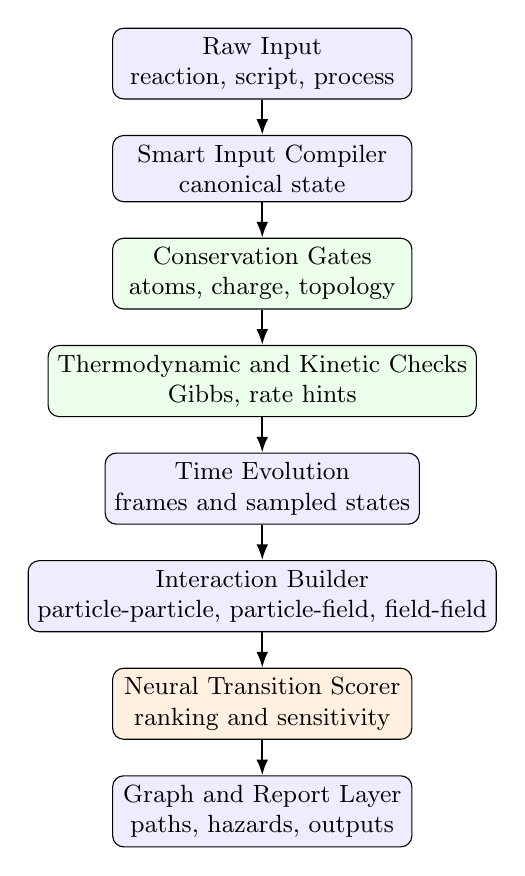
\begin{tikzpicture}[
  node distance=0.45cm,
  every node/.style={font=\small},
  stage/.style={draw, rounded corners, align=center, minimum width=3.8cm, minimum height=0.78cm, fill=blue!7},
  gate/.style={draw, rounded corners, align=center, minimum width=3.8cm, minimum height=0.78cm, fill=green!8},
  model/.style={draw, rounded corners, align=center, minimum width=3.8cm, minimum height=0.78cm, fill=orange!12},
  arrow/.style={-{Latex[length=2mm]}, thick}
]
\node[stage] (raw) {Raw Input\\reaction, script, process};
\node[stage, below=of raw] (compile) {Smart Input Compiler\\canonical state};
\node[gate, below=of compile] (conserve) {Conservation Gates\\atoms, charge, topology};
\node[gate, below=of conserve] (thermo) {Thermodynamic and Kinetic Checks\\Gibbs, rate hints};
\node[stage, below=of thermo] (frames) {Time Evolution\\frames and sampled states};
\node[stage, below=of frames] (interactions) {Interaction Builder\\particle-particle, particle-field, field-field};
\node[model, below=of interactions] (score) {Neural Transition Scorer\\ranking and sensitivity};
\node[stage, below=of score] (report) {Graph and Report Layer\\paths, hazards, outputs};

\draw[arrow] (raw) -- (compile);
\draw[arrow] (compile) -- (conserve);
\draw[arrow] (conserve) -- (thermo);
\draw[arrow] (thermo) -- (frames);
\draw[arrow] (frames) -- (interactions);
\draw[arrow] (interactions) -- (score);
\draw[arrow] (score) -- (report);
\end{tikzpicture}
\caption{High-level data flow from raw input to ranked transition report.}
\end{figure}

% ---------------------------------------------------------------------------
\section{Basic Reactivity Modeling}

The first layer is basic reactivity modeling. It does not require a neural network. It requires clean inputs, structured parsing, and chemistry-aware validation.

A basic reaction model should answer:

\begin{itemize}[leftmargin=1.2cm]
  \item Are the species syntactically valid?
  \item Are atoms conserved?
  \item Is charge conserved?
  \item Is the reaction family recognizable?
  \item Is the product set chemically plausible?
  \item Is the reaction thermodynamically favored?
  \item Is the reaction kinetically accessible?
\end{itemize}

A minimal reaction input may look like:

\begin{lstlisting}[caption={Raw reaction input}]
CH4 + 2O2 -> CO2 + 2H2O
\end{lstlisting}

The compiler converts that string into a structured representation:

\begin{lstlisting}[caption={Structured reaction representation}]
reactants:
  CH4: 1
  O2: 2

products:
  CO2: 1
  H2O: 2

reaction_type:
  combustion

environment:
  temperature: unknown
  pressure: unknown
  phase: gas_or_unknown
\end{lstlisting}

The first serious rule of the system is therefore:

\begin{quote}
\textbf{The neural network does not override conservation laws.}
\end{quote}

The model may score, classify, rank, or suggest. It does not get to vote against atom balance, charge balance, or basic physical constraints.

% ---------------------------------------------------------------------------
\section{Reaction Time as a Core Variable}

A reaction is not merely:

\begin{lstlisting}
reactants -> products
\end{lstlisting}

It is more accurately represented as:

\begin{lstlisting}
reactants(t0) -> intermediates(t1...tn) -> products(tf)
\end{lstlisting}

Time must therefore become a first-class variable. Important time-related values include reaction time, time step, sampling interval, half-life estimate, rate constant, activation delay, mixing time, thermal ramp time, cooling time, diffusion time, and residence time.

\begin{table}[H]
\centering
\caption{Example time-resolved combustion state}
\begin{tabular}{rrrrr}
\toprule
Time (s) & \ce{CH4} & \ce{O2} & \ce{CO2} & \ce{H2O}\\
\midrule
0.0 & 1.0 & 2.0 & 0.0 & 0.0\\
0.5 & 0.7 & 1.4 & 0.3 & 0.6\\
1.0 & 0.2 & 0.4 & 0.8 & 1.6\\
1.5 & 0.0 & 0.0 & 1.0 & 2.0\\
\bottomrule
\end{tabular}
\end{table}

Each time sample becomes a frame. Every frame can be checked, scored, graphed, and used as training material.

\begin{figure}[H]
\centering
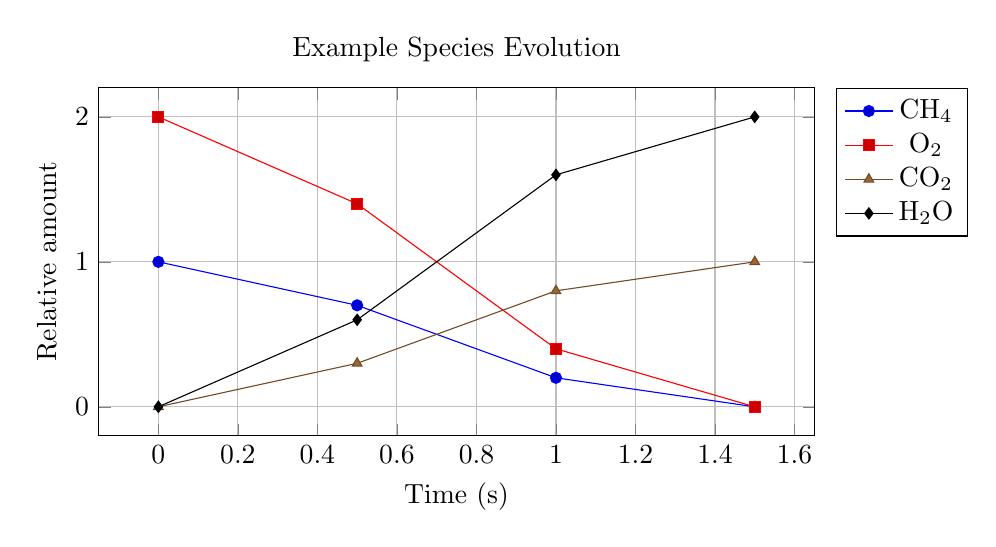
\begin{tikzpicture}
\begin{axis}[
  width=0.88\linewidth,
  height=6cm,
  xlabel={Time (s)},
  ylabel={Relative amount},
  title={Example Species Evolution},
  grid=major,
  legend pos=outer north east
]
\addplot+[mark=*] coordinates {(0,1.0) (0.5,0.7) (1.0,0.2) (1.5,0.0)};
\addlegendentry{\ce{CH4}}
\addplot+[mark=square*] coordinates {(0,2.0) (0.5,1.4) (1.0,0.4) (1.5,0.0)};
\addlegendentry{\ce{O2}}
\addplot+[mark=triangle*] coordinates {(0,0.0) (0.5,0.3) (1.0,0.8) (1.5,1.0)};
\addlegendentry{\ce{CO2}}
\addplot+[mark=diamond*] coordinates {(0,0.0) (0.5,0.6) (1.0,1.6) (1.5,2.0)};
\addlegendentry{\ce{H2O}}
\end{axis}
\end{tikzpicture}
\caption{Illustrative time evolution of reactants and products.}
\end{figure}

% ---------------------------------------------------------------------------
\section{Functional Programming Model}

The reaction system should be built from small composable functions rather than one monolithic solver.

\begin{lstlisting}[caption={Composable pipeline functions}]
parse_reaction()
balance_check()
charge_check()
classify_reaction()
estimate_gibbs()
estimate_rate()
run_md_check()
apply_thermal_step()
generate_frame()
graph_outputs()
score_transition()
\end{lstlisting}

The reaction becomes a chain of transformations:

\begin{lstlisting}[caption={Functional transformation chain}]
raw_string
  -> parsed_reaction
  -> algebra_checked_reaction
  -> thermodynamic_checked_reaction
  -> md_checked_reaction
  -> time_evolved_reaction
  -> graphed_reaction
  -> model_ready_transition
\end{lstlisting}

A simplified execution flow is:

\begin{lstlisting}[caption={Simplified implementation sketch}]
reaction = parse_reaction(raw_input)

reaction = algebra_check(reaction)
reaction = gibbs_check(reaction)
reaction = md_check(reaction)

frames = thermal_time_evolve(reaction, delta_t)

graphs = generate_graphs(frames)
scores = neural_transition_score(frames)
\end{lstlisting}

This modular structure prevents invalid candidates from being promoted blindly into later, more expensive stages.

% ---------------------------------------------------------------------------
\section{Algebra and Charge Checks}

The algebra check verifies atom and charge conservation. For combustion of methane:

\[
\ce{CH4 + 2O2 -> CO2 + 2H2O}
\]

\begin{table}[H]
\centering
\caption{Atom balance for balanced methane combustion}
\begin{tabular}{lrrr}
\toprule
Element & Reactants & Products & Delta\\
\midrule
C & 1 & 1 & 0\\
H & 4 & 4 & 0\\
O & 4 & 4 & 0\\
\bottomrule
\end{tabular}
\end{table}

A failed candidate can still be retained, but it must be labeled honestly.

\begin{lstlisting}[caption={Failed candidate labeling}]
reaction: CH4 + O2 -> CO2 + H2O
atom_balance: fail
charge_balance: pass
candidate_status: invalid_candidate
training_value: negative_example
\end{lstlisting}

This is useful because the learning system benefits from both successful and failed candidates.

% ---------------------------------------------------------------------------
\section{Thermodynamic Screening}

After algebra, the next major gate is Gibbs free energy screening. The simplified criterion is:

\[
\Delta G < 0 \Rightarrow \text{thermodynamically favorable}
\]
\[
\Delta G = 0 \Rightarrow \text{equilibrium}
\]
\[
\Delta G > 0 \Rightarrow \text{thermodynamically unfavorable}
\]

The early system does not require a complete thermodynamic database. It can begin with symbolic categories:

\begin{lstlisting}[caption={Symbolic Gibbs categories}]
strongly_favorable
weakly_favorable
near_equilibrium
unfavorable
unknown
\end{lstlisting}

For methane combustion, the expected classification is:

\begin{lstlisting}[caption={Example thermodynamic classification}]
reaction: CH4 + 2O2 -> CO2 + 2H2O
gibbs_direction: favorable
energy_behavior: exothermic
reaction_family: combustion
thermodynamic_plausibility: high
kinetic_accessibility: condition_dependent
\end{lstlisting}

The Gibbs layer produces an evidence attribute rather than a final verdict. Some reactions are thermodynamically possible but kinetically blocked.

% ---------------------------------------------------------------------------
\section{Molecular-Dynamics Plausibility Check}

The molecular-dynamics check moves the system from symbolic chemistry toward simulation-aware chemistry. Its early purpose is not to solve every bond-breaking event. Instead, it acts as a geometry, energy, and stability filter.

\begin{lstlisting}[caption={MD plausibility questions}]
Are the starting structures stable?
Are candidate products stable?
Are reactive sites spatially accessible?
Do particles collide under sampled conditions?
Does the system relax without numerical failure?
Does thermal input destabilize expected bonds?
Do intermediate arrangements look plausible?
\end{lstlisting}

A minimal MD output may look like:

\begin{lstlisting}[caption={Example MD validation output}]
initial_geometry_stable: true
product_geometry_stable: true
collision_accessible: true
relaxation_success: true
high_energy_artifacts: false
\end{lstlisting}

A frame-based output can expose energy and force trends:

\begin{lstlisting}[caption={Example frame-based MD output}]
frame_0000:
  total_energy: -102.4
  max_force: 0.18
  geometry_status: stable

frame_0050:
  total_energy: -91.2
  max_force: 0.44
  geometry_status: activated

frame_0100:
  total_energy: -128.7
  max_force: 0.12
  geometry_status: relaxed_product
\end{lstlisting}

% ---------------------------------------------------------------------------
\section{Thermal Evolution and \texorpdfstring{$\Delta t$}{delta-t}}

Thermal evolution applies controlled state updates:

\[
state(t + \Delta t) = thermal\_update(state(t), T, P, fields, \Delta t)
\]

The thermal stepping model should track temperature, pressure, species amounts, reaction progress, energy, stability, and rate estimate.

\begin{lstlisting}[caption={Thermal stepping loop}]
for each frame:
    apply_temperature()
    update_species_amounts()
    update_reaction_progress()
    update_energy()
    check_stability()
    save_frame()
\end{lstlisting}

Possible graph outputs include concentration versus time, temperature versus time, reaction progress versus time, Gibbs estimate versus time, potential energy versus frame, stability score versus frame, and field strength versus reaction rate.

% ---------------------------------------------------------------------------
\section{Batch Frame Generation}

A single reaction should not remain a single datapoint. The batch engine runs many variations of the same base transition.

\begin{lstlisting}[caption={Batch variation targets}]
temperature
pressure
concentration
reaction_time
mixing
field_strength
catalyst_presence
geometry
initial_velocity
\end{lstlisting}

A batch result may look like:

\begin{lstlisting}[caption={Example batch definitions}]
reaction_batch_001:
  frames: 500
  temperature_distribution: normal
  pressure_distribution: normal
  concentration_distribution: normal
  catalyst: none
  output: stable_combustion_path

reaction_batch_002:
  frames: 500
  temperature_distribution: high_tail
  pressure_distribution: elevated
  concentration_distribution: oxygen_limited
  output: incomplete_combustion_path
\end{lstlisting}

The reaction becomes a cloud of outcomes rather than one fixed symbolic transformation.

% ---------------------------------------------------------------------------
\section{Variable Sweeping}

The system should vary parameters using distributions rather than unstructured randomness. For many ordinary operating conditions, normal distributions are useful:

\[
T \sim \mathcal{N}(\mu_T,\sigma_T)
\]
\[
P \sim \mathcal{N}(\mu_P,\sigma_P)
\]

Other distributions are appropriate when the variable demands it: log-normal for rate constants, uniform sampling for broad screening, bimodal sampling for phase transitions, heavy-tail distributions for rare extremes, and discrete sampling for catalyst selection.

\begin{figure}[H]
\centering
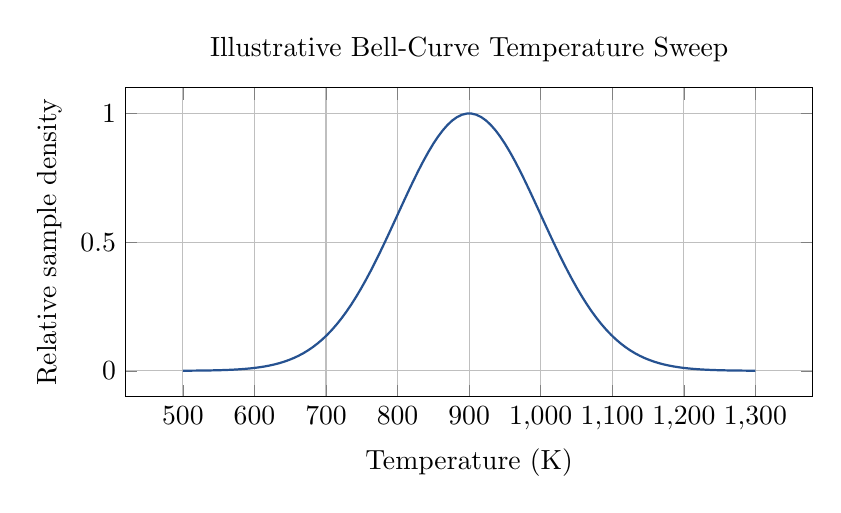
\begin{tikzpicture}
\begin{axis}[
  width=0.85\linewidth,
  height=5.5cm,
  xlabel={Temperature (K)},
  ylabel={Relative sample density},
  title={Illustrative Bell-Curve Temperature Sweep},
  grid=major,
  domain=500:1300,
  samples=120
]
\addplot[thick, stageblue] {exp(-((x-900)^2)/(2*100^2))};
\end{axis}
\end{tikzpicture}
\caption{Example normal sampling around a nominal combustion temperature of 900 K.}
\end{figure}

The output should identify stable regions, unstable regions, fast paths, slow paths, high-yield regions, low-yield regions, sensitive variables, and likely failure modes.

% ---------------------------------------------------------------------------
\section{Isomer Sorting}

After candidate products are generated or supplied, the system should sort possible isomers. A formula is not a structure.

For example, \ce{C2H6O} can correspond to ethanol or dimethyl ether.

\begin{table}[H]
\centering
\caption{Example isomer sorting output}
\begin{tabular}{lllll}
\toprule
Formula & Candidate & Family & Stability & Notes\\
\midrule
\ce{C2H6O} & Ethanol & Alcohol & High & Bio-relevant, moderate volatility\\
\ce{C2H6O} & Dimethyl ether & Ether & High & Higher volatility\\
\bottomrule
\end{tabular}
\end{table}

The system must track connectivity, bond order, geometry, functional groups, stability, reaction family, biological relevance, toxicity flags, and likely artifacts.

% ---------------------------------------------------------------------------
\section{Biological and Safety Screening}

Advanced reaction outputs should include biological and safety screening. This is not a substitute for toxicology databases or laboratory review. It is a screening layer.

Possible flags include:

\begin{lstlisting}[caption={Safety screening channels}]
bioactivity_possible
known_functional_group_risk
reactive_group_flag
toxicity_hint
volatility_hint
corrosivity_hint
flammability_hint
environmental_persistence_hint
bioaccumulation_hint
\end{lstlisting}

Example:

\begin{lstlisting}[caption={Example safety flag output}]
candidate_product:
  formula: C6H6
  name: benzene

bio_check:
  biological_risk: high
  toxicity_flag: true
  aromatic_hydrocarbon: true
  handling_risk: high
\end{lstlisting}

The pipeline should distinguish between chemical plausibility, industrial usefulness, biological safety, and environmental acceptability.

% ---------------------------------------------------------------------------
\section{Transition from Toy System to Serious System}

The early system can parse reactions, check algebra, estimate Gibbs direction, run simplified MD checks, sweep variables, generate frames, sort isomers, screen biological flags, and graph outcomes. That is already useful.

The advanced system treats reactions as evolving high-dimensional interaction systems. The input is no longer merely reactants, products, and conditions. It becomes particles, fields, surfaces, geometries, energies, gradients, constraints, time evolution, candidate paths, and learned transition pressures.

% ---------------------------------------------------------------------------
\section{Field-Aware Reaction Reasoning}

A reaction environment is not empty space. It may include thermal, pressure, electric, magnetic, radiation, concentration, flow, phase, solvent, surface, and chemical-potential fields.

Each particle can affect fields. Each field can affect particles. Fields can also affect one another. This produces three major interaction classes:

\begin{itemize}[leftmargin=1.2cm]
  \item particle-particle interactions,
  \item particle-field interactions,
  \item field-field interactions.
\end{itemize}

The state can be represented as an interaction tensor:

\[
\mathcal{I} =
\left\{
I_{PP}, I_{PF}, I_{FF}
\right\}
\]

where \(I_{PP}\) describes particle-particle relations, \(I_{PF}\) describes particle-field coupling, and \(I_{FF}\) describes field-field coupling.

\begin{figure}[H]
\centering
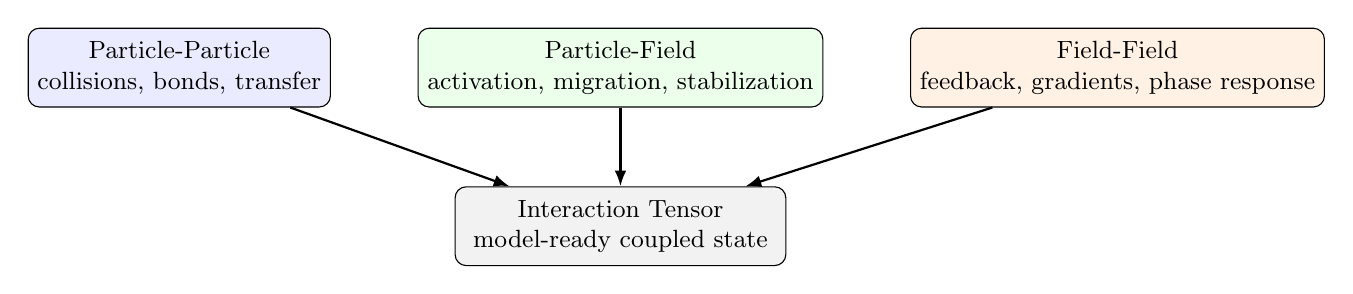
\begin{tikzpicture}[
  block/.style={draw, rounded corners, align=center, minimum width=3.2cm, minimum height=1cm},
  arrow/.style={-{Latex[length=2mm]}, thick},
  every node/.style={font=\small}
]
\node[block, fill=blue!8] (pp) {Particle-Particle\\collisions, bonds, transfer};
\node[block, fill=green!8, right=1.1cm of pp] (pf) {Particle-Field\\activation, migration, stabilization};
\node[block, fill=orange!10, right=1.1cm of pf] (ff) {Field-Field\\feedback, gradients, phase response};

\node[block, fill=gray!10, below=1cm of pf, minimum width=4.2cm] (tensor) {Interaction Tensor\\model-ready coupled state};

\draw[arrow] (pp) -- (tensor);
\draw[arrow] (pf) -- (tensor);
\draw[arrow] (ff) -- (tensor);
\end{tikzpicture}
\caption{Interaction tensor built from particle-particle, particle-field, and field-field relations.}
\end{figure}

% ---------------------------------------------------------------------------
\section{Particle-Particle Interactions}

Particle-particle interactions describe relationships between chemical entities. These can include collision likelihood, bond rearrangement possibility, electron transfer, steric accessibility, reactive-site alignment, distance distribution, relative velocity, local energy, and orientation factor.

\begin{lstlisting}[caption={Example particle-particle feature packet}]
interaction: CH4 <-> O2

oxidation_possible: true
requires_activation: true
radical_pathway_possible: true
bond_breaking_required: high
bond_forming_reward: high
orientation_dependency: medium
\end{lstlisting}

This allows the model to learn from physical relationships instead of symbolic reaction names alone.

% ---------------------------------------------------------------------------
\section{Particle-Field Interactions}

Particle-field interactions describe how species respond to the environment.

\begin{lstlisting}[caption={Particle-field examples}]
O2 <-> thermal_field:
  radical_support: medium
  activation_support: medium
  high_temperature_reactivity: increased

Na+ <-> electric_field:
  migration_response: high
  orientation_effect: low
  field_coupling: strong

organic_intermediate <-> solvent_field:
  polarity_stabilization: high
  transition_state_support: condition_dependent
\end{lstlisting}

A reaction under vacuum, water, plasma, molten salt, catalyst bed, or biological fluid should not be treated as the same event.

% ---------------------------------------------------------------------------
\section{Field-Field Interactions}

Field-field interactions describe environmental coupling. Thermal gradients affect pressure. Pressure affects phase. Flow affects concentration. Radiation affects ionization, which can alter electric response and pathway accessibility.

\begin{lstlisting}[caption={Field-field examples}]
thermal_field <-> pressure_field:
  coupling_strength: high
  rate_modifier: strong
  phase_risk: medium

flow_field <-> concentration_field:
  coupling_strength: high
  mixing_dependency: strong
  local_depletion_risk: high
\end{lstlisting}

This layer is especially important for industrial systems. A reaction in a vessel is chemistry plus heat transfer, pressure response, flow, mixing, wall effects, residence time, and control behavior.

% ---------------------------------------------------------------------------
\section{Neural Scoring Layer}

The neural network should sit after deterministic checks and interaction construction. It should receive structured feature packets, not raw strings.

\begin{lstlisting}[caption={Model-ready feature packet}]
conservation_features
thermodynamic_features
kinetic_features
topology_features
field_features
interaction_tensor_features
time_series_features
graph_features
safety_features
isomer_features
\end{lstlisting}

The neural scorer can output plausibility, reaction-family scores, pathway scores, stability scores, field-sensitivity scores, hazard scores, yield likelihood, and failure likelihood.

\begin{lstlisting}[caption={Example neural scoring output}]
candidate: methane_combustion_path_A

overall_plausibility: 0.94
reaction_family: combustion
yield_likelihood: 0.91
field_sensitivity: medium
hazard_score: high_temperature_risk
failure_likelihood: 0.06
recommended_next_check: detailed_thermal_run
\end{lstlisting}

% ---------------------------------------------------------------------------
\section{Candidate Universe Generation}

The advanced system should not evaluate only one candidate reaction. It should generate and rank a universe of possible transitions.

\begin{lstlisting}[caption={Candidate-generation pipeline}]
initial_state
  -> candidate_generator
  -> algebra_filter
  -> Gibbs_filter
  -> topology_filter
  -> MD_filter
  -> field_interaction_filter
  -> isomer_sort
  -> bio_safety_check
  -> neural_ranker
  -> final_transition_set
\end{lstlisting}

The output becomes a ranked map of likely main reactions, possible side reactions, unstable branches, condition-sensitive branches, hazardous branches, biologically relevant branches, high-yield regions, and failure regions.

% ---------------------------------------------------------------------------
\section{High-Dimensional Batch Reasoning}

The full system operates across high-dimensional batches. Each batch may vary temperature, pressure, time, concentration, geometry, field strength, flow, mixing, catalyst, surface area, phase, solvent, radiation, electric potential, magnetic influence, initial velocity, and molecular orientation.

The full batch is collapsed into summary maps:

\begin{lstlisting}[caption={Batch summary maps}]
yield_map
stability_map
hazard_map
energy_map
pathway_map
field_sensitivity_map
isomer_distribution_map
bio_relevance_map
failure_map
\end{lstlisting}

Example output:

\begin{lstlisting}[caption={Example process-region summary}]
main_product_favored:
  temperature: 820-930 K
  pressure: 1.0-1.3 atm
  oxygen_ratio: 1.8-2.2
  mixing: high

side_product_risk_increases:
  oxygen_ratio: < 1.4
  temperature: < 750 K
  residence_time: too_short

thermal_runaway_risk_increases:
  temperature: > 1100 K
  pressure: > 1.5 atm
  heat_removal: poor
\end{lstlisting}

% ---------------------------------------------------------------------------
\section{Graph-Level Learning}

Eventually, individual feature vectors may not be enough. Reactions are graphs. Molecules are graphs. Vessels and pipes are graphs. Frames over time form graph sequences.

A molecular graph tracks atoms as nodes, bonds as edges, bond order as edge attributes, charges as node attributes, and geometry as spatial attributes.

A process graph tracks vessels as nodes, pipes as edges, flow as edge attributes, temperature and pressure as node states, and reaction zones as active nodes.

A reaction graph tracks reactants, intermediates, products, transition edges, energy barriers, and field coupling.

The eventual form is:

\begin{lstlisting}[caption={Graph-level transition form}]
state_graph + operator_graph + field_graph + time_frames
  -> transition_scores
\end{lstlisting}

At this point, the system is no longer merely classifying reactions. It is modeling evolving structured physical systems.

% ---------------------------------------------------------------------------
\section{Full Target Architecture}

The final target is a chemical process intelligence layer. It accepts reaction strings, molecular structures, process scripts, pipe and vessel layouts, field definitions, thermal schedules, batch parameters, candidate products, environmental constraints, and safety constraints.

It produces validated reactions, ranked pathways, time-evolved frames, graphs, isomer maps, field interaction maps, bio/safety flags, industrial process summaries, failure modes, and model-ready training packets.

\begin{lstlisting}[caption={Full target architecture}]
Raw Input
  -> Smart Input Compiler
  -> Canonical Chemical/Process State
  -> Algebra and Conservation Checks
  -> Thermodynamic Checks
  -> Kinetic and MD Checks
  -> Time Evolution
  -> Batch Sampling
  -> Isomer Sorting
  -> Bio/Safety Screening
  -> Interaction Tensor Builder
  -> Neural Transition Scorer
  -> Graph Output Layer
  -> Final Ranked Transition Report
\end{lstlisting}

The difference between a classroom reaction checker and an off-scale chemical reasoning engine is the difference between asking whether a reaction is balanced and asking which physically plausible paths a system can follow under specific constraints.

% ---------------------------------------------------------------------------
\section{Development Strategy}

The system should be built in phases. Each phase produces useful outputs by itself and also generates cleaner input for the next phase.

\begin{longtable}{p{0.11\linewidth} p{0.78\linewidth}}
\caption{Phased development plan}\\
\toprule
Phase & Deliverables\\
\midrule
\endfirsthead
\toprule
Phase & Deliverables\\
\midrule
\endhead
1 & String parser, species table, stoichiometry parser, algebra check, charge check, basic reaction-family classification.\\
2 & Gibbs estimate, energy direction, basic kinetic hints, temperature and pressure context, graph outputs.\\
3 & Time frames, thermal stepping, batch generation, bell-curve variable sweeps, reaction-progress graphs.\\
4 & Isomer sorting, candidate product generation, biological and safety screening, hazard flags.\\
5 & Particle-particle interactions, particle-field interactions, field-field interactions, interaction tensor.\\
6 & Hardcoded neural network, transition scoring, candidate ranking, active learning from failed and successful runs.\\
7 & Graph learning, process graph support, pipe/vessel coupling, field-aware industrial simulation.\\
\bottomrule
\end{longtable}

\begin{figure}[H]
\centering
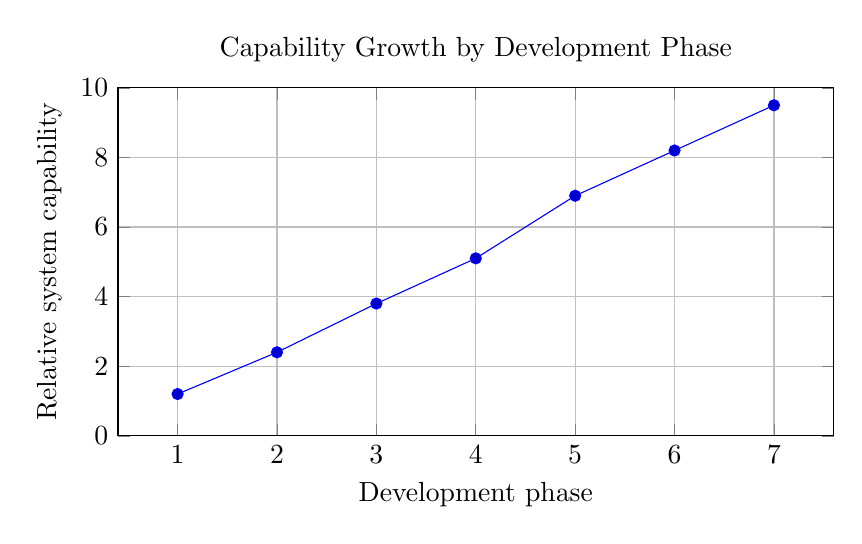
\begin{tikzpicture}
\begin{axis}[
  width=0.88\linewidth,
  height=6cm,
  xlabel={Development phase},
  ylabel={Relative system capability},
  title={Capability Growth by Development Phase},
  ymin=0,
  ymax=10,
  xtick={1,2,3,4,5,6,7},
  grid=major
]
\addplot+[mark=*] coordinates {
  (1,1.2)
  (2,2.4)
  (3,3.8)
  (4,5.1)
  (5,6.9)
  (6,8.2)
  (7,9.5)
};
\end{axis}
\end{tikzpicture}
\caption{Illustrative capability curve across the proposed development phases.}
\end{figure}

% ---------------------------------------------------------------------------
\section{Program Output Targets}

A shareable version of the project should include program outputs. These outputs should be short in the main report and complete in an appendix or external log directory.

\begin{lstlisting}[caption={Example CLI output for a successful transition check}]
$ vsim chem check methane_combustion.vsim

[parse] reaction loaded: CH4 + 2O2 -> CO2 + 2H2O
[balance] atom balance: pass
[balance] charge balance: pass
[classify] family: combustion
[thermo] Gibbs direction: favorable
[kinetics] accessibility: condition_dependent
[frames] generated: 500
[batch] sampled conditions: 128
[safety] hazard flags: high_temperature, flammable_feed
[result] status: accepted_candidate
\end{lstlisting}

\begin{lstlisting}[caption={Example CLI output for a failed candidate}]
$ vsim chem check malformed_combustion.vsim

[parse] reaction loaded: CH4 + O2 -> CO2 + H2O
[balance] atom balance: fail
[balance] delta C: 0
[balance] delta H: -2
[balance] delta O: +1
[result] status: invalid_candidate
[result] training_label: negative_example
\end{lstlisting}

These outputs make the project inspectable. The report should show what the program did, not merely describe what the program is supposed to do.

% ---------------------------------------------------------------------------
\section{Recommended Shareable Package}

The project should be distributed as a small reproducible packet:

\begin{lstlisting}[caption={Recommended shareable directory layout}]
smart-reaction-learning-pipeline/
|-- README.md
|-- report/
|   `-- smart_reaction_learning_pipeline.tex
|-- scripts/
|   |-- methane_combustion.vsim
|   |-- oxygen_limited_combustion.vsim
|   `-- isomer_sort_c2h6o.vsim
|-- outputs/
|   |-- methane_combustion_output.txt
|   |-- failed_balance_output.txt
|   `-- batch_summary.txt
|-- data/
|   |-- species_time_series.csv
|   |-- batch_sweep.csv
|   `-- candidate_scores.csv
`-- figures/
    |-- species_time_series.pdf
    |-- phase_capability.pdf
    `-- candidate_ranking.pdf
\end{lstlisting}

The minimum defensible public packet is:

\begin{lstlisting}
README.md
report.pdf
report.tex
scripts/
outputs/
figures/
\end{lstlisting}

% ---------------------------------------------------------------------------
\section{Validation Checklist}

A future implementation should be able to report the following validation status.

\begin{table}[H]
\centering
\caption{Validation checklist}
\begin{tabular}{lll}
\toprule
Validation item & Expected result & Purpose\\
\midrule
Parser accepts valid reaction & Pass & Confirms input compiler behavior\\
Parser rejects malformed species & Pass & Prevents invalid state construction\\
Atom balance check & Pass/fail label & Enforces conservation\\
Charge balance check & Pass/fail label & Enforces electrochemical validity\\
Gibbs screen & Direction label & Adds thermodynamic prior\\
Frame generator & Stable frames & Enables time-series output\\
Batch sampler & Distribution summary & Enables parameter sweep\\
Isomer sorter & Ranked candidates & Prevents formula-only reasoning\\
Safety screen & Flags & Adds handling and biological caution\\
Neural scorer & Ranked paths & Evaluates structured transitions\\
\bottomrule
\end{tabular}
\end{table}

% ---------------------------------------------------------------------------
\section{Conclusion}

The \pipeline{} should begin as a small deterministic checker and grow into a structured chemical process reasoning engine. The architecture intentionally separates hard constraints from learned scoring. Conservation laws, charge balance, topology, thermodynamic evidence, molecular-dynamics plausibility, and safety flags form the scaffold. Neural scoring then ranks physically structured transition candidates rather than guessing from raw strings.

The first version can be small. The architecture should not be. The system becomes powerful by compiling chemical reality into structured, inspectable, graphable states before any learning layer is trusted with ranking the next transition.

\appendix

% ---------------------------------------------------------------------------
\section{Appendix A: Minimal Example Script}

\begin{lstlisting}[caption={Example input script for methane combustion}]
[reaction]
name = "methane_combustion"
equation = "CH4 + 2O2 -> CO2 + 2H2O"
family_hint = "combustion"

[environment]
temperature_K = 900
pressure_atm = 1.0
phase = "gas"

[batch]
frames = 500
temperature_mean_K = 900
temperature_sigma_K = 100
pressure_mean_atm = 1.0
pressure_sigma_atm = 0.1

[outputs]
write_species_graph = true
write_energy_graph = true
write_candidate_scores = true
\end{lstlisting}

% ---------------------------------------------------------------------------
\section{Appendix B: Example CSV Outputs}

\begin{lstlisting}[caption={Example species time series CSV}]
time_s,CH4,O2,CO2,H2O
0.0,1.0,2.0,0.0,0.0
0.5,0.7,1.4,0.3,0.6
1.0,0.2,0.4,0.8,1.6
1.5,0.0,0.0,1.0,2.0
\end{lstlisting}

\begin{lstlisting}[caption={Example candidate scores CSV}]
candidate,plausibility,yield_likelihood,hazard_score
main_combustion_path,0.94,0.91,0.72
oxygen_limited_path,0.71,0.56,0.84
stalled_low_temp_path,0.38,0.22,0.31
runaway_high_temp_path,0.64,0.48,0.96
\end{lstlisting}

% ---------------------------------------------------------------------------
\section{Appendix C: Notes for Future Integration}

Future integration work should connect this design to real parser outputs, real thermochemical data sources, real graph serialization, generated fixtures, and regression tests. The report should then replace illustrative outputs with captured program outputs from the current build.

\end{document}
